\documentclass{beamer}
\usepackage{moreverb} 
\usepackage{listings}
\usepackage{mflogo}
% imprimir
% \documentclass[handout]{beamer} 
% \usepackage{pgfpages}
% \pgfpagesuselayout{4 on 1}[a4paper,landscape,border shrink=5mm]

\mode<presentation> {
  \usetheme{Warsaw}
  \setbeamercovered{opaque}
}

\usebackgroundtemplate{
\includegraphics[width=\paperwidth]{format/libresoft-bg.png}}
\usepackage[spanish]{babel}
\usepackage[utf8]{inputenc}
\usepackage{graphics}
\usepackage{amssymb} % Simbolos matematicos

%% Metadatos del PDF.
\hypersetup{  
  pdftitle={StaaS: el almacenamiento como servicio},
  pdfauthor={Miguel Vidal},
  pdfcreator={GSyC/Libresoft},
  pdfproducer=PDFLaTeX,
  pdfsubject={Master on Free Software},
}
%%

\defbeamertemplate*{footline}{shadow theme}
{%
  \leavevmode%
  \hbox{\begin{beamercolorbox}[wd=.5\paperwidth,ht=2.5ex,dp=1.125ex,leftskip=.1cm plus1fil,rightskip=.2cm]{author in head/foot}%

\includegraphics[scale=0.40]{format/cc-by-80x15.png} \hspace{0.05cm}
	Miguel Vidal / Jose Castro
  \end{beamercolorbox}%
  \begin{beamercolorbox}[wd=.5\paperwidth,ht=2.5ex,dp=1.125ex,leftskip=.3cm,rightskip=.3cm plus1fil]{title in head/foot}%
    \usebeamerfont{title in head/foot}\insertshorttitle%
    \hspace{2cm} \usebeamerfont{author in head/foot}\insertframenumber\,/\,\inserttotalframenumber\hfill
  \end{beamercolorbox}}%
  \vskip0pt%
}


\begin{document}

\title{StaaS: el almacenamiento como servicio (II)}
\subtitle{System Integration}
% \institute{\texttt{http://gsyc.urjc.es/\~{}mvidal} \\ Twitter: \texttt{@mvidallopez}}
\author{Miguel Vidal, Jose Castro} 
\date{\footnotesize{Master on Free Software \\ March 30th, 2012}}
\author{Miguel Vidal \hspace{1cm} Jose Castro \\
\hspace{0.5mm} {\tiny Twitter: @mvidallopez \hspace{1.1cm}Twitter: @jfcastroluis}
}


\frame{
\maketitle
\begin{center}

\includegraphics[width=6cm]{format/gsyc-urjc}
\end{center}
}

%% License slide
\begin{frame}
  \vspace{2cm}
  \begin{flushright}
    {\small \copyright{} 2010-2012 Miguel Vidal, Jose Castro} \\
%    \vspace{0.25cm}
    \medskip
    {\scriptsize This work is licensed under \\ a Creative Commons Attribution 3.0 License}
%    \vspace{0.10cm}
  \end{flushright}
  \begin{flushright}
    \href{http://creativecommons.org/licenses/by/3.0/es}{
\includegraphics[width=2cm]{format/cc-by.png}} \\
    {\tiny \url{http://creativecommons.org/licenses/by/3.0}}
  \end{flushright}
\end{frame}%%

\usebackgroundtemplate{}

\AtBeginSection[]
{
\begin{frame}<beamer>
\begin{center}
{\huge \insertsection}
\end{center}
\end{frame}
}


\AtBeginSubsection[]
{
  \begin{frame}<beamer>{Índice}
    \tableofcontents[currentsection,currentsubsection]
  \end{frame}
}

%%


\section{Almacenamiento por red}

\subsection{NAS/SAN}

\begin{frame}
  \frametitle{Network-Attached Storage (NAS)}
  \begin{itemize}
    \item Almacenamiento de datos \alert{orientados a fichero}.
    \item Exportación de recursos (sistema de ficheros) vía red a clientes heterogéneos.
    \item El cliente solicita el fichero completo al servidor y lo maneja localmente.
    \item Protocolos antiguos e inseguros (aunque NFSv4 mejora seguridad y rendimiento). 
	  \begin{itemize}
	    \item \alert{NFS} (Network Filesystem): muy usado en sistemas Unix, aunque también disponible en muchos otros. 
	    \item \alert{CIFS/SMB} (Common Internet File System): Muy popular en redes Windows. Implementado libremente para Unixes con \alert{Samba}.
	  \end{itemize}

  \end{itemize}
\end{frame}

\begin{frame}
  \frametitle{Storage Area Network (SAN)}

\begin{figure}[h]
\begin{center}
  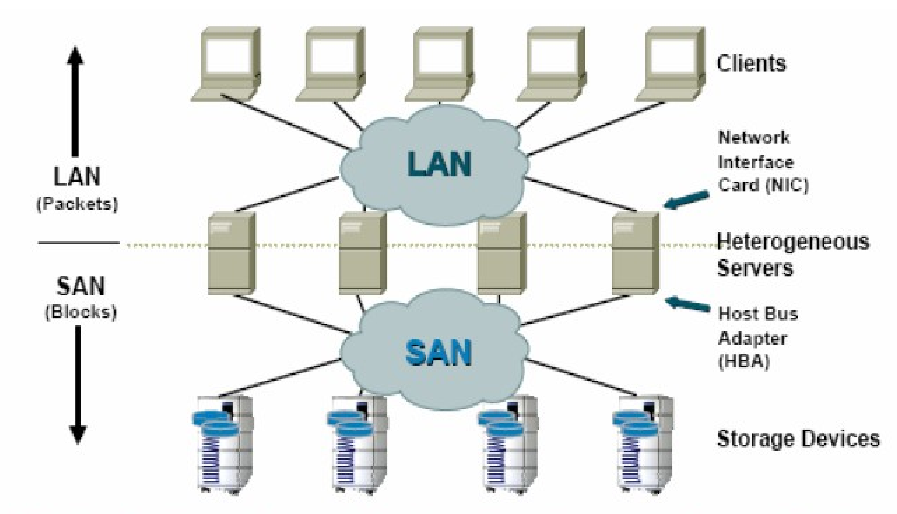
\includegraphics[width=6.75cm]{figs/SAN.png}
%  \caption{{\footnotesize SAN is a dedicated network for attaching servers to storage devices.}}
\end{center}
\end{figure}

  \begin{itemize}
    \item Opera solamente a \alert{nivel de bloque}. 
     \item SAN deja todo lo relacionado con el sistema de ficheros al ``cliente''.
    \item Los protocolos SAN: SCSI, Fibre Channel, iSCSI, ATA over Ethernet (AoE), o HyperSCSI.
  \end{itemize}


\end{frame}


\begin{frame}
  \frametitle{iSCSI}
  \begin{itemize}
    \item Almacenamiento por red basado en IP.
    \item Es un popular y relativamente nuevo protocolo SAN (opera a nivel de bloque).
    \item  iSCSI se compone de dos elementos:
  \begin{enumerate}
	\item Initiator
	\item Target
  \end{enumerate}
    \item Los clientes (\alert{initiators}) envían los comandos SCSI (CDBs) a los dispositivos de almacenamiento SCSI (\alert{targets}) a través de redes IP.
    \item A diferencia del tradicional Fibre Channel, no requiere infraestructura o cableado especial.
  \end{itemize}
\end{frame}

\begin{frame}
  \frametitle{ATA over Ethernet: almacenamiento de bajo coste}

\begin{figure}[h]
\begin{center}
  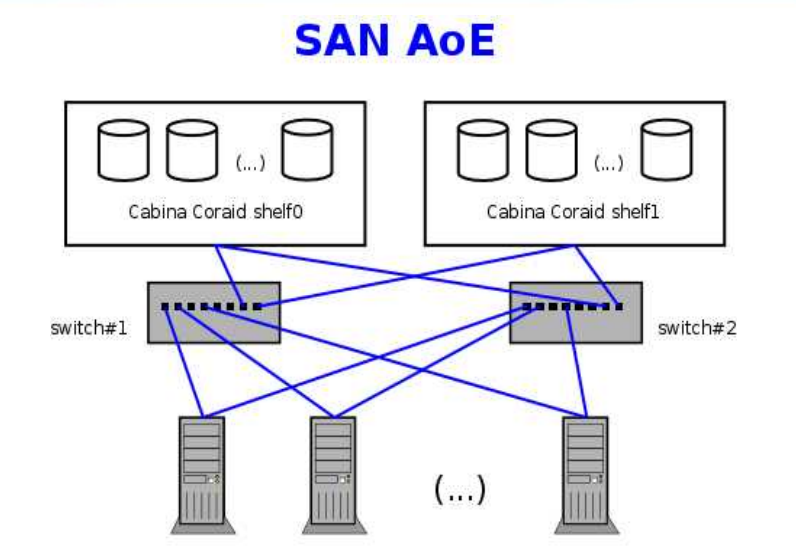
\includegraphics[width=9cm]{figs/san_aoe.png}
\end{center}
\end{figure}

\end{frame}


\begin{frame}
  \frametitle{NAS vs. SAN}
  \begin{itemize}
\small
    \item NAS provee al mismo tiempo el almacenamiento y el sistema de ficheros.
    \item SAN provee solo almacenamiento a nivel de bloque y deja que el cliente se encargue de lo relativo al FS.  
    \item Diferentes protocolos.
    \item SAN y NAS no son excluyentes, pueden combinarse.
  \end{itemize}

\normalsize

\begin{figure}[h]
\begin{center}
  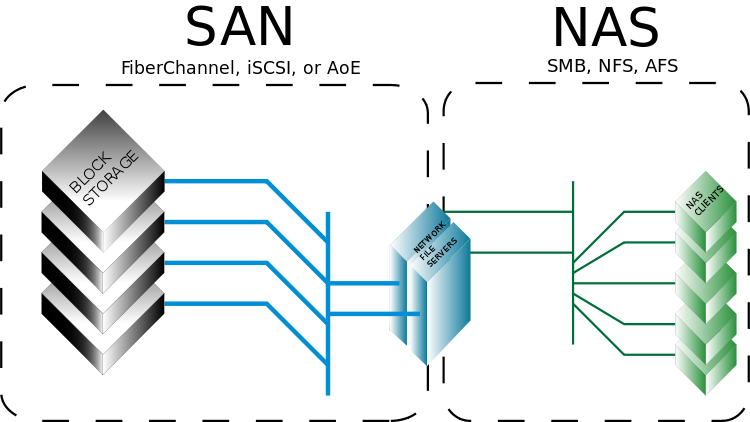
\includegraphics[width=6cm]{figs/SANvsNAS.png}
\end{center}
\end{figure}

\end{frame}

\subsection{Replicación de disco}

\begin{frame}
  \frametitle{Replicación del almacenamiento de disco}
  \begin{itemize}
    \item El método más básico es el \alert{mirror de disco}, típico para discos conectados localmente.
	  \begin{itemize}
	    \item \alert{replicación síncrona:} sin pérdida (``zero data loss''), operaciones atómicas de escritura (ACK),
	    \item \alert{Replicación asíncrona}: larga distancia, latencia alta. Incrementa el rendimiento, pero en caso de pérdida, no se garantiza que el almacenamiento remoto tenga copia actualizada de los datos.
	  \end{itemize}
    \item DRBD para Linux. 
    \item AVS para derivados de Solaris.
  \end{itemize}
\end{frame}

\begin{frame}
  \frametitle{DRBD}
  \begin{itemize}
    \item DRBD: \textit{Distributed Replicated Block Device}: mirror (raid-1) de discos sobre LAN.
    \item Sistema de replicación para Linux: parte oficial del kernel desde 2.6.33.
    \item Con frecuencia desplegado en combinación con Heartbeat (Linux HA).
    \item Datos solo accesibles en nodo activo (salvo que se use un FS paralelo como GFS u OCFS2).

  \end{itemize}
\end{frame}


\begin{frame}
  \frametitle{Arquitectura de DRBD}

\begin{figure}[h]
\begin{center}
  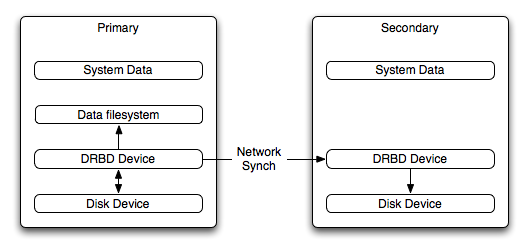
\includegraphics[width=10cm]{figs/drbd-main.png}
\end{center}
\end{figure}

\end{frame}

\begin{frame}
  \frametitle{Arquitectura de AVS}

Sun StorageTek Availability Suite, replicación remota con *Solaris:

\begin{figure}[h]
\begin{center}
  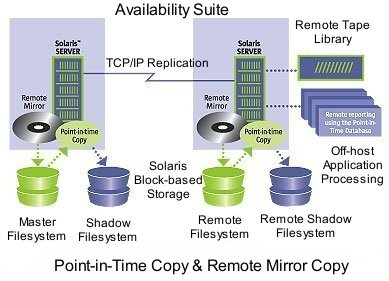
\includegraphics[width=8cm]{figs/availabilitysuitenew.jpg}
\end{center}
\end{figure}

\end{frame}

\subsection{Sistemas de ficheros distribuidos}
\begin{frame}
  \frametitle{Sistemas de fichero distribuido}

\begin{center}
\textbf{¿Que pasa si tenemos un DRBD en 2 equipos y queremos montar al mismo tiempo la misma partición?}
\end{center}

\pause
  \begin{itemize}
    \item Los \alert{FS tradicionales no lo permiten}: necesario FS de tipo clúster (``distribuido'', ``paralelo'' o ''compartido'').
    \item Se forma un cluster propio entre los nodos que pueden montar el FS compartido.
    \item Soportan montaje y \alert{acceso concurrente desde varios nodos} a la vez: evita corrupción de datos cuando se accede a los ficheros desde diferentes hosts.
  \end{itemize}
\end{frame}

\begin{frame}
  \frametitle{Sistemas de ficheros distribuidos}

  \begin{itemize}

    \item A diferencia del NFS, que exporta directorios, \alert{se exportan como un filesystem completo}. 
    \item Ejemplos: OCFS2, GFS (Global File System, no confundir con Google FS).

    \item Desventajas:

  \begin{itemize}
	\item Sistemas más complejos de configurar y de mantener.
	\item Rendimiento inferior.
  \end{itemize}

  \end{itemize}
\end{frame}

\begin{frame}
  \frametitle{Sistemas de ficheros distribuidos: GlusterFS}

  \begin{itemize}
    \item Cliente/servidor: 
	  \begin{itemize}
	  \item El \alert{servidor} NAS exporta filesystem como volúmenes. 
	  \item El \alert{cliente} se conecta por TCP/IP o Infiniband y compone volúmenes en espacio de usuario (libglusterfs o FUSE) a través de \alert{traductores}.
          \item Los \alert{traductores} conectan uno o más subvolúmenes e incluyen las funcionalidades (mirror, stripping, balanceo de carga, cuotas, etc.)
	  \end{itemize}
    \item Evita el cuello de botella por múltiple concurrencia. No se compromete rendimiento.
    \item Muy simple. Apto para cloud.

  \end{itemize}
\end{frame}


\begin{frame}
  \frametitle{Sistemas de ficheros distribuidos: GlusterFS}
\vspace{-0.25cm}
\begin{figure}[h]
\begin{center}
  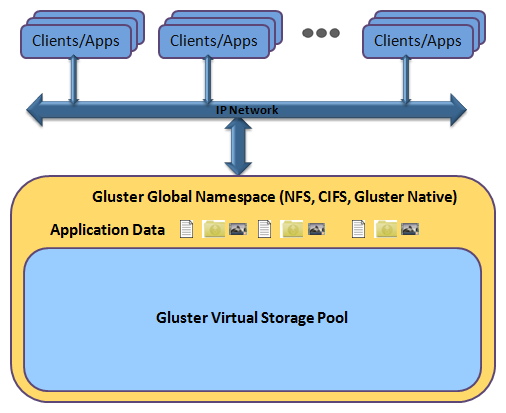
\includegraphics[width=7.5cm]{figs/diagram-glusterfs.png}
  \caption{GlusterFS -- Un punto de montaje común}
\end{center}
\end{figure}

\end{frame}


\subsection{StaaS}
\begin{frame}
  \frametitle{StaaS: Virtualización del almacenamiento}
  \begin{itemize}
    \item Abstracción transparente del almacenamiento físico.
    \item Los recursos de almacenamiento físico se agregan en \alert{pools}, desde los que se crea el almacenamiento lógico.
    \item Implementado en los modernos arrays de disco.
    \item \alert{Storage as a Service}: la separación (abstracción) permite incrementar la flexibilidad a los SysAdmins. 
    \item StaaS es parte de soluciones \alert{cloud}, \alert{clustering} y \alert{HA}.
  \end{itemize}
\end{frame}


%%%%%%%%%section%%%%%%%%%%%%%%

\section{Backups}

\subsection{Aspectos generales}

\begin{frame}
  \frametitle{Aspectos generales (1)}
  \begin{itemize}
    \item Proteger los datos es una de las tareas más importantes de un sysadmin.
    \item Desafortunadamente es también una de las tareas más tediosas.

    \item Los backups deben hacerse con cuidado y estrictamente planificados.
  \end{itemize}
\end{frame}

\begin{frame}
  \frametitle{Aspectos generales (y 2)}
  \begin{itemize}
    \item El sistema de backups y los medios de almacenamiento deben verificarse regularmente.
    \item Los sistemas de backups NO deben confundirse con sistemas tolerantes a fallos.
    \item La integridad de los medio de backup es vital y afecta directamente al balance de una empresa. 
  \end{itemize}
\end{frame}


\begin{frame}
  \frametitle{Métodos de backup}
  \begin{itemize}
    \item \alert{No estructurados:} una pila de discos o CD-R/DVD-R con mínima información sobre lo que fue respaldado y cuándo. 
    \item \alert{backups incrementales:} backups sucesivos que contienen solamente los cambios desde el último backup.
	  \begin{itemize}
		\item Una forma óptima de ahorrar espacio. Es muy eficiente
		\item Diferentes implementaciones.
	  \end{itemize}
  \end{itemize}
\end{frame}

\begin{frame}
  \frametitle{Métodos de backup (y 2)}
  \begin{itemize}
    \item \alert{Backups diferenciales:} coge todos los ficheros que han cambiado desde el último backup completo (\textit{full}). La restauración requiere disponer del último backup completo.
    \item \alert{Backup completo:} para ser recuperado completamente desde cero. 
    \item \alert{Protección continua de datos:} no se planifican backups periódicos, el sistema registra cada cambio de forma inmediata en el sistema anfitrión.
  \end{itemize}
\end{frame}



\subsection{rsync}
\begin{frame}
  \frametitle{\texttt{rsync}: transferir ficheros de forma segura}
  \begin{itemize}
    \item Puede sincronizar ficheros y directorios de una máquina a otra y puede ejecutarse junto con SSH para transferir datos de forma segura por la Red.
    \item Opcionalmente, dispone de compresión y recursión.
    \item Muy \textit{scriptable}: Similar a \texttt{scp} pero es más escrupuloso a la hora de preservar links, fechas y permisos.
    \item Procura transmitir solo diferencias entre versiones.
    \item Forma parte del sistema base de muchas distribuciones. Es ampliamente usado.
  \end{itemize}
\end{frame}


\subsection{Bacula}

\begin{frame}
  \frametitle{Bacula}
  \begin{itemize}
    \item Bacula es una solución cliente/servidor de nivel empresarial que gestiona backups, restauración y verificación de ficheros a través de una red.
    \item Bacula corre en en Linux y en diversos Unixes.
    \item Dispone de agentes que permiten respaldar datos de muchos SOs, incluido Microsoft Windows.
  \end{itemize}
\end{frame}


\begin{frame}
  \frametitle{Componentes de Bacula}

\begin{figure}[h]
\begin{center}
  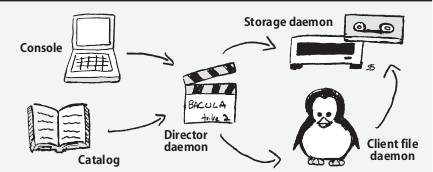
\includegraphics[width=7.5cm]{figs/bacula.png}
%  \caption 
\end{center}
\end{figure}

  \begin{itemize}

    \item \alert{Bacula director}: demonio que coordina las operaciones de respaldo, restauración y verificación.
    \item \alert{Bacula console}: permite enviar trabajos manualmente al \texttt{director} para que los restaure o respalde. 
    \item Un \alert{demonio cliente de Bacula} corre en cada sistema que debe ser respaldado.
  \end{itemize}

\end{frame}

%%%%%%%%%%%%%%%%%%%%%%%%%%%%%%%%%%%%%%%%%%%%%%%%%%%%%%%%%%%%%%%%%%%%%%%%%

% Portada final
\frame{
\maketitle
\begin{center}

\includegraphics[width=6cm]{format/gsyc-urjc}
\end{center}
}


%Fin de la presentacion
\end{document}


